%8
\documentclass[12pt, oneside]{article}

\usepackage[letterpaper, scale=0.89, centering]{geometry}
\usepackage{fancyhdr}
\setlength{\parindent}{0em}
\setlength{\parskip}{1em}

\pagestyle{fancy}
\fancyhf{}
\renewcommand{\headrulewidth}{0pt}
\rfoot{\href{https://creativecommons.org/licenses/by-nc-sa/2.0/}{CC BY-NC-SA 2.0} Version \today~(\thepage.)}

\usepackage{amssymb,amsmath,pifont,amsfonts,comment,enumerate}
\usepackage{currfile,xstring,hyperref,tabularx,graphicx,wasysym}
\usepackage[labelformat=empty]{caption}
\usepackage[dvipsnames,table]{xcolor}
\usepackage{multicol,multirow,array,listings,tabularx,lastpage,textcomp,booktabs}

% NOTE(joe): This environment is credit @pnpo (https://tex.stackexchange.com/a/218450)
\lstnewenvironment{algorithm}[1][] %defines the algorithm listing environment
{   
    \lstset{ %this is the stype
        mathescape=true,
        frame=tB,
        numbers=left, 
        numberstyle=\tiny,
        basicstyle=\rmfamily\scriptsize, 
        keywordstyle=\color{black}\bfseries,
        keywords={,procedure, div, for, to, input, output, return, datatype, function, in, if, else, foreach, while, begin, end, }
        numbers=left,
        xleftmargin=.04\textwidth,
        #1
    }
}
{}
\lstnewenvironment{java}[1][]
{   
    \lstset{
        language=java,
        mathescape=true,
        frame=tB,
        numbers=left, 
        numberstyle=\tiny,
        basicstyle=\ttfamily\scriptsize, 
        keywordstyle=\color{black}\bfseries,
        keywords={, int, double, for, return, if, else, while, }
        numbers=left,
        xleftmargin=.04\textwidth,
        #1
    }
}
{}

\newcommand\abs[1]{\lvert~#1~\rvert}
\newcommand{\st}{\mid}

\newcommand{\A}[0]{\texttt{A}}
\newcommand{\C}[0]{\texttt{C}}
\newcommand{\G}[0]{\texttt{G}}
\newcommand{\U}[0]{\texttt{U}}

\newcommand{\cmark}{\ding{51}}
\newcommand{\xmark}{\ding{55}}



\begin{document}
\begin{flushright}
    \StrBefore{\currfilename}{.}
\end{flushright}

\section*{Monday February 22}
%! app: TODOapp
%! outcome: TODOoutcome

\begin{tabular}{clc}
    $\mathbb{Z}$ &  The  set of integers  & $\{ \ldots, -2, -1, 0,  1, 2, \ldots\}$ \\
    $\mathbb{Z}^+$ &  The  set of positive integers  & $\{1, 2, \ldots\}$ \\
    $\mathbb{N}$ &  The  set of nonnegative integers  & $\{0, 1, 2, \ldots\}$ \\
    $\mathbb{Q}$ &  The  set of rational numbers  & $\left\{ \frac{p}{q} \mid p \in \mathbb{Z}  \text{ and  } q  \in \mathbb{Z} \text{ and } q \neq  0 \right\}$\\
    $\mathbb{R}$ & The  set  of  real numbers &  \\
    \end{tabular}
    \[
    \underline{\phantom{\mathbb{Z}^+}} ~~\subsetneq~~ \underline{\phantom{\mathbb{N}~}} ~~\subsetneq ~~\underline{\phantom{\mathbb{Z}~}}~~ \subsetneq~~ \underline{\phantom{\mathbb{Q}~}} 
    ~~\subsetneq~~ \underline{\phantom{\mathbb{R}~}} 
    \]
    
    
    The above sets are all {\bf infinite}.
    
    
    A {\bf finite} set is one whose distinct elements can be counted by a natural number.
    
    {\it Examples of finite sets}: $\emptyset$ , $\{ \sqrt{2} \}$
    
    
    {\bf Motivating question}: Are some of the above sets {\it bigger than} others?
{\it Analogy}: Musical chairs

\begin{multicols}{2}
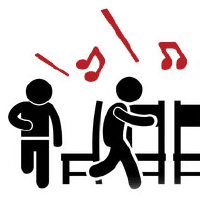
\includegraphics[width=2in]{../../resources/images/musicalChairs.png}
\columnbreak

People try to sit down when the music stops

Person\sun~ sits in Chair 1,
Person\smiley~ sits in Chair 2,

Person\frownie~  is left standing!
\end{multicols}
What does this say about the number of chairs and the number of people?
\vfill
\fbox{\parbox{\textwidth}{%
{\bf Defining functions} A function is defined by its (1) domain, (2) codomain, and (3) rule assigning each 
element in the domain exactly one element in the codomain. The domain and codomain are nonempty sets.
The rule can be depicted as a table, formula, English description, etc.\\

(Rosen p139)
}}


{\it Example}: $f_A: \mathbb{R}^+ \to \mathbb{Q}$ with $f_A(x) = x$ is {\bf not} a well-defined function because

\vfill


{\it Example}: $f_B: \mathbb{Q} \to \mathbb{Z}$ with $f_B\left(\frac{p}{q}\right) = p+q$ is {\bf not} a well-defined function because

\vfill


{\it Example}: $f_C: \mathbb{Z} \to \mathbb{R}$ with $f_C(x) = \frac{x}{|x|}$ is {\bf not} a well-defined function because
\newpage
{\bf Definition}  (Rosen p141): A function $f: D  \to C$ is {\bf one-to-one} (or  injective) means for every $a,b$ in the domain $D$, 
if $f(a) = f(b)$ then  $a=b$.

{\bf Definition}:  For sets $A, B$, we say that  {\bf the  cardinality of $A$ is  no  bigger than the cardinality of  $B$}, and 
write $|A| \leq |B|$, to mean there is a  one-to-one function  with domain $A$  and codomain $B$.
{\it In the analogy}: The function $sitter: \{ Chair1, Chair2\} \to \{ Person\sun, Person\smiley, Person\frownie \}$ given
by $sitter(Chair1) = Person\sun$,  $sitter(Chair2) = Person\smiley$, is one-to-one and witnesses that 
\[
| \{ Chair1, Chair2\} | \leq |\{ Person\sun, Person\smiley, Person\frownie \}|
\]
%! app: TODOapp
%! outcome: TODOoutcome

Let $S_2$ be the set of RNA strands of length 2.

\vspace{-20pt}

\begin{center}
\begin{tabular}{|c|p{5in}|}
\hline
Statement  &  True/False , justification \\
\hline
$| \{\A,\U,\G,\C\} | \leq |S_2 |$ &  \\
&\\&\\&\\
\hline
$| \{\A,\U,\G,\C\} \times \{\A, \U, \G,\C\} | \leq |S_2 |$ &  \\
&\\&\\&\\
\hline
\end{tabular}
\end{center}
%! app: TODOapp
%! outcome: TODOoutcome

{\bf Definition}: A function $f: D  \to C$ is {\bf onto} (or  surjective) means for every $b$ in the codomain, 
there  is an element $a$ in the domain with  $f(a) = b$.


Formally, $f: D  \to  C$ is  onto  means $\underline{\phantom{\forall b \in C  \exists a \in D ( f(a) = b)}}$.


{\bf Definition}:  For sets $A, B$, we say that  {\bf the  cardinality of $A$ is  no  smaller than the cardinality of  $B$}, and 
write $|A| \geq |B|$, to mean there is an onto function  with domain $A$  and codomain $B$.

%! app: TODOapp
%! outcome: TODOoutcome

{\it In the analogy}: The function $triedToSit: \{ Person\sun, Person\smiley, Person\frownie \} \to  \{ Chair1, Chair2\} $ given
by $triedToSit(Person\sun) = Chair1$,  $triedToSit(Person\smiley) = Chair2$, 
$triedToSit(Person\frownie) = Chair2$, is onto and witnesses that 
\[
 |\{ Person\sun, Person\smiley, Person\frownie \}| \geq | \{ Chair1, Chair2\} |
\]
%! app: TODOapp
%! outcome: TODOoutcome

Let $S_2$ be the set of RNA strands of length 2.

{\bf True} or {\bf False}: $ |S_2 | \geq | \{\A,\U,\G,\C\} |$

{\it Why?}
\vspace{80pt}

{\bf True} or {\bf False}: $ |S_2 | \geq | \{\A,\U,\G,\C\} \times \{\A, \U, \G,\C\} |$

{\it Why?}
\vspace{80pt}
\newpage
{\bf Definition}  (Rosen p144): A function $f: D  \to C$ is a {\bf bijection} means that it is both  one-to-one  and onto.
The {\bf inverse} of a  bijection $f: D  \to  C$ is  the function $g: C  \to  D$  such that $g(b) = a$ iff  $f(a) =  b$.


\fbox{\parbox{\textwidth}{%
For nonempty sets $A, B$ we say
\begin{align*}
|A| \leq |B| &\text{ means there is a one-to-one function with domain $A$, codomain $B$} \\
|A| \geq |B| &\text{ means there is an onto function with domain $A$, codomain $B$} \\
|A| = |B| &\text{ means there is a bijection with domain $A$, codomain $B$}
\end{align*}
}}
%! app: TODOapp
%! outcome: TODOoutcome

{\bf Properties of cardinality}
\begin{align*}
&\forall A ~ (~  |A| = |A| ~)\\
&\forall A ~ \forall B ~(~ |A| = |B|  ~\to ~ |B| = |A|~)\\
&\forall A ~ \forall B ~ \forall C~ (~ (|A| = |B| ~\wedge~ |B| = |C|) ~\to ~ |A| = |C|~)
\end{align*}

{\it Extra practice with proofs:} Use the definitions of bijections to prove these properties.
\vfill
%! app: TODOapp
%! outcome: TODOoutcome

{\bf Cantor-Schroder-Bernstein Theorem}: For all nonempty sets,
\[
|A| = |B| \qquad\text{if and only if} \qquad (|A| \leq |B| ~\text{and}~ |B| \leq |A|)
\qquad\text{if and only if} \qquad (|A| \geq |B| ~\text{and}~ |B| \geq |A|)
\]

To prove $|A| = |B|$,  we can do any {\bf one} of the following

\begin{itemize}\setlength{\itemsep}{-5pt}
\item Prove there exists  a bijection $f:  A \to B$;
\item Prove there exists a  bijection  $f: B  \to  A$;
\item Prove there exists two functions $f_1: A \to B$, $f_2: B \to  A$ where each of $f_1, f_2$ is one-to-one.
\item Prove there exists two functions $f_1: A \to B$, $f_2: B \to  A$ where each of $f_1, f_2$ is onto.
\end{itemize}


\end{document}